\documentclass[12pt,a4paper]{report}

% Packages
\usepackage[utf8]{inputenc}
\usepackage[T1]{fontenc}
\usepackage{amsmath}
\usepackage{amssymb}
\usepackage[lining]{ebgaramond}
\usepackage[cmintegrals,cmbraces]{newtxmath}
\usepackage{microtype}
\usepackage{geometry}
\usepackage{graphicx}
\usepackage{booktabs}
\usepackage{array}
\usepackage{xcolor}
\usepackage{hyperref}
\usepackage{float}
\usepackage{caption}
\usepackage{etoolbox}
\usepackage{enumitem}
\usepackage{makecell}
\graphicspath{{./fig/}}

% Page layout
\geometry{
    left=1.8cm,
    right=1.8cm,
    top=2.2cm,
    bottom=2.2cm
}

% Color definitions
\definecolor{crimson}{RGB}{153, 0, 0}

% Hyperlink settings
\hypersetup{
    colorlinks=true,
    linkcolor=crimson,
    urlcolor=crimson,
    citecolor=crimson
}

\tolerance=2000
\emergencystretch=2em

% Chapter/section title formatting
\usepackage{titlesec}
\titleformat{\chapter}{\normalfont\huge\bfseries}{}{0pt}{}[\vspace{0.3em}]
\titlespacing*{\chapter}{0pt}{0pt}{14pt}
\titleformat{\section}{\normalfont\Large\bfseries}{\thesection}{1em}{}
\titleformat{\subsection}{\normalfont\large\bfseries}{\thesubsection}{1em}{}

\setlength{\parindent}{0pt}
\setlength{\parskip}{4pt}

% Float spacing
\setlength{\floatsep}{6pt plus 2pt minus 2pt}
\setlength{\textfloatsep}{10pt plus 2pt minus 2pt}
\setlength{\intextsep}{10pt plus 2pt minus 2pt}
\setlength{\abovecaptionskip}{4pt}
\setlength{\belowcaptionskip}{0pt}
\captionsetup[figure]{skip=5pt, belowskip=2pt}
\captionsetup[table]{skip=2pt}
\BeforeBeginEnvironment{figure}{\vspace{4pt}}
\AfterEndEnvironment{figure}{\vspace{2pt}}
\AfterEndEnvironment{table}{\vspace{-6pt}}

% Question box: \question{text}
\newcommand{\question}[1]{%
    \hrule
    \vspace{0.2cm}
    #1
    \vspace{0.2cm}
    \hrule
    \vspace{0.5cm}
}

\newcommand{\Tsym}{T_{sym}}

\begin{document}

\pagestyle{plain}

% ─────────────────────────────────────────────
%  Cover Page
% ─────────────────────────────────────────────
\begin{titlepage}
\centering
\vspace*{3cm}

{\fontsize{28}{34}\selectfont\bfseries Digital Communication IC Design\par}
\vspace{0.6em}
{\fontsize{20}{26}\selectfont\bfseries Homework 1\par}

\vspace{1.5cm}
\textcolor{crimson}{\rule{0.6\linewidth}{1.2pt}}
\vspace{1.5cm}

{\large\bfseries Student ID}\par
\vspace{0.4em}
{\large M11407439}\par

\vspace{0.8em}

{\large\bfseries Name}\par
\vspace{0.4em}
{\large MING-HONG, LIN}\par

\vspace{2cm}

{\large\bfseries Development Environment}\par
\vspace{0.8em}
\begin{tabular}{rl}
    \textbf{Language} & MATLAB R2025b \\[4pt]
    \textbf{AI Tool}  & Claude Opus 5.5 \\
\end{tabular}

\vfill

\textcolor{crimson}{\rule{0.6\linewidth}{0.6pt}}\par
\vspace{0.5em}
{\small Due Date: 2026/10/07}

\end{titlepage}

% ─────────────────────────────────────────────
%  Table of Contents
% ─────────────────────────────────────────────
\tableofcontents
\newpage

% ─────────────────────────────────────────────
\chapter{Random Binary Data}
% ─────────────────────────────────────────────
\section{Generated Bits}

\question{Please randomly generate 32 binary bits by using your last two digits as the seed, and
print out your own bits ($b_i$, $i = 0, 1, \ldots, 31$). These binary data will be used throughout
homework 1.}

The bits are generated once in \texttt{01\_src/gen\_bits.m} and shared by all three questions:

\begin{center}
\texttt{rng(39, 'twister');\quad b = randi([0 1], 1, 32);}
\end{center}

\begin{table}[H]
\centering
\caption{Random Bits $b_0 \sim b_{31}$ (seed $= 39$)}
\setlength{\tabcolsep}{5pt}
\renewcommand{\arraystretch}{1.2}
\begin{tabular}{c*{16}{c}}
\toprule
$i$   & 0 & 1 & 2 & 3 & 4 & 5 & 6 & 7 & 8 & 9 & 10 & 11 & 12 & 13 & 14 & 15 \\
$b_i$ & 1 & 1 & 1 & 0 & 1 & 1 & 0 & 0 & 1 & 1 & 1  & 1  & 1  & 0  & 1  & 1  \\
\midrule
$i$   & 16 & 17 & 18 & 19 & 20 & 21 & 22 & 23 & 24 & 25 & 26 & 27 & 28 & 29 & 30 & 31 \\
$b_i$ & 1  & 0  & 1  & 1  & 0  & 1  & 1  & 0  & 0  & 1  & 1  & 0  & 1  & 0  & 1  & 1  \\
\bottomrule
\end{tabular}
\end{table}

\newpage

% ─────────────────────────────────────────────
\chapter{Q1 — Single-Carrier QPSK and O-QPSK}
% ─────────────────────────────────────────────
All waveforms in Q1 use the settings below. The QPSK symbol $a_k$ comes from the black points
in Fig.~1 of the spec, which sit on the unit circle at odd multiples of $\pi/4$:
\begin{equation}
    a_k = \frac{(1 - 2b_{2k}) + j\,(2b_{2k+1} - 1)}{\sqrt{2}},
    \qquad (0,1) \to 45^\circ,\ (1,1) \to 135^\circ,\ (1,0) \to 225^\circ,\ (0,0) \to 315^\circ .
\end{equation}

\begin{table}[H]
\centering
\caption{Single-Carrier Simulation Settings}
\setlength{\tabcolsep}{10pt}
\renewcommand{\arraystretch}{1.2}
\begin{tabular}{lcl}
\toprule
\textbf{Quantity} & \textbf{Value} & \textbf{Derived interpretation} \\
\midrule
Symbol period $\Tsym$      & 0.1\,\textmu s & 10\,Msymbol/s, 16 symbols in total \\
Carrier frequency $f_c$    & 40\,MHz        & 4 carrier cycles per symbol \\
Sampling frequency $f_s$   & 640\,MHz       & 16 samples per carrier cycle \\
Samples per symbol         & 64             & half-symbol delay $=$ 32 samples \\
\bottomrule
\end{tabular}
\end{table}

\begin{table}[H]
\centering
\caption{QPSK Symbols $a_k$ Mapped from $(b_{2k}, b_{2k+1})$}
\setlength{\tabcolsep}{8pt}
\renewcommand{\arraystretch}{1.2}
\begin{tabular}{cccc}
\toprule
$k$ & $(b_{2k}, b_{2k+1})$ & $a_k$ & $\angle a_k$ \\
\midrule
0 & (1, 1) & $(-1+j)/\sqrt{2}$ & $135^\circ$ \\
1 & (1, 0) & $(-1-j)/\sqrt{2}$ & $225^\circ$ \\
2 & (1, 1) & $(-1+j)/\sqrt{2}$ & $135^\circ$ \\
3 & (0, 0) & $(+1-j)/\sqrt{2}$ & $315^\circ$ \\
4 & (1, 1) & $(-1+j)/\sqrt{2}$ & $135^\circ$ \\
5 & (1, 1) & $(-1+j)/\sqrt{2}$ & $135^\circ$ \\
6 & (1, 0) & $(-1-j)/\sqrt{2}$ & $225^\circ$ \\
7 & (1, 1) & $(-1+j)/\sqrt{2}$ & $135^\circ$ \\
\bottomrule
\end{tabular}
\hspace{2em}
\begin{tabular}{cccc}
\toprule
$k$ & $(b_{2k}, b_{2k+1})$ & $a_k$ & $\angle a_k$ \\
\midrule
8  & (1, 0) & $(-1-j)/\sqrt{2}$ & $225^\circ$ \\
9  & (1, 1) & $(-1+j)/\sqrt{2}$ & $135^\circ$ \\
10 & (0, 1) & $(+1+j)/\sqrt{2}$ & $45^\circ$ \\
11 & (1, 0) & $(-1-j)/\sqrt{2}$ & $225^\circ$ \\
12 & (0, 1) & $(+1+j)/\sqrt{2}$ & $45^\circ$ \\
13 & (1, 0) & $(-1-j)/\sqrt{2}$ & $225^\circ$ \\
14 & (1, 0) & $(-1-j)/\sqrt{2}$ & $225^\circ$ \\
15 & (1, 1) & $(-1+j)/\sqrt{2}$ & $135^\circ$ \\
\bottomrule
\end{tabular}
\end{table}

\newpage

\section{(a) QPSK Baseband Signal}

\question{Define $p(t) = 1$ for $0 \le t < \Tsym$ and $0$ otherwise, and generate the complex baseband
QPSK signal by using the mapping of the black points defined in Fig.~1 as $a_k$, where the constellation
points lie on the unit circle. Plot its real and imaginary parts. Note that the x-axis should be expressed
in \textmu s and $t$ starts from 0. (5\%)
\[ x_{BB,QPSK}(t) = \sum_{k=0}^{15} a_k\, p(t - k\Tsym) \]}

With a rectangular $p(t)$, $x_{BB}(t)$ just holds $a_k$ for the whole $k$-th symbol.
I repeat each symbol for 64 samples ($f_s = 640$\,MHz), which gives 1024 samples over
$0 \le t < 1.6$\,\textmu s. The real part $I(t) = \pm 1/\sqrt{2}$ is set by $b_{2k}$ and the imaginary part
$Q(t) = \pm 1/\sqrt{2}$ by $b_{2k+1}$. Both rails can flip at the same boundary, which becomes
important in Q1(g).

\begin{figure}[H]
    \centering
    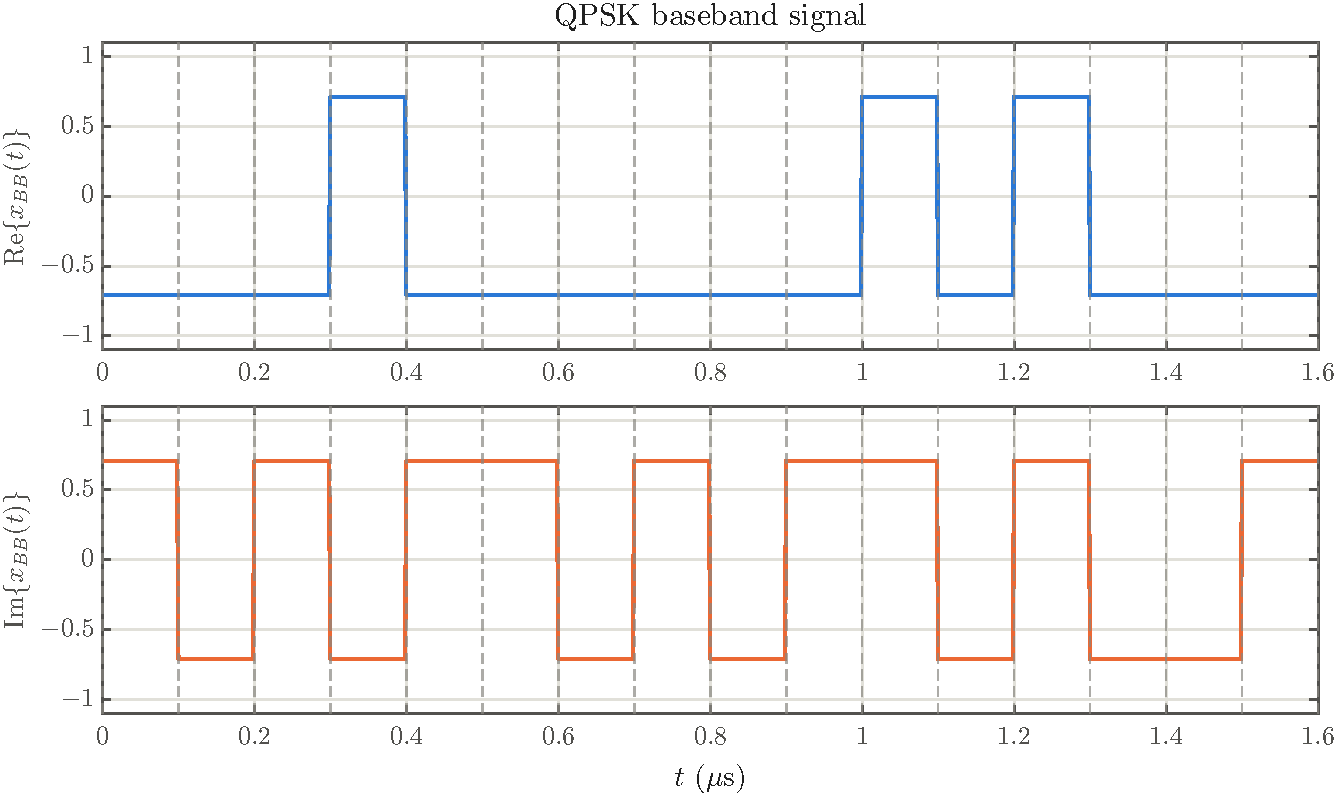
\includegraphics[width=0.9\linewidth]{q1a.pdf}
    \caption{Real and Imaginary Parts of the QPSK Baseband Signal (gray dashed lines: symbol boundaries)}
\end{figure}

\newpage

\section{(b) Passband Signal}

\question{Upconvert the baseband waveform to the real passband signal as defined in the course slides.
Plot the first eight symbol periods and mark all symbol boundaries with vertical black dashed lines. (10\%)}

Following the QPSK definition in the course slides (Chapter~2, p.~16), the real passband signal is
\begin{equation}
    x_{PB}(t) = \mathrm{Re}\left\{ x_{BB}(t)\, e^{j2\pi f_c t} \right\}
              = I(t)\cos(2\pi f_c t) - Q(t)\sin(2\pi f_c t).
\end{equation}
Since $|a_k| = 1$, the envelope stays constant and $x_{PB}(t)$ is a 40\,MHz cosine with phase $\angle a_k$.
Each symbol holds exactly $f_c \Tsym = 4$ carrier cycles. Whenever $a_k$ changes, the carrier phase
breaks at the boundary; the clearest cases are $t = 0.3$ and $0.4$\,\textmu s, where the phase jumps by $\pi$.

\begin{figure}[H]
    \centering
    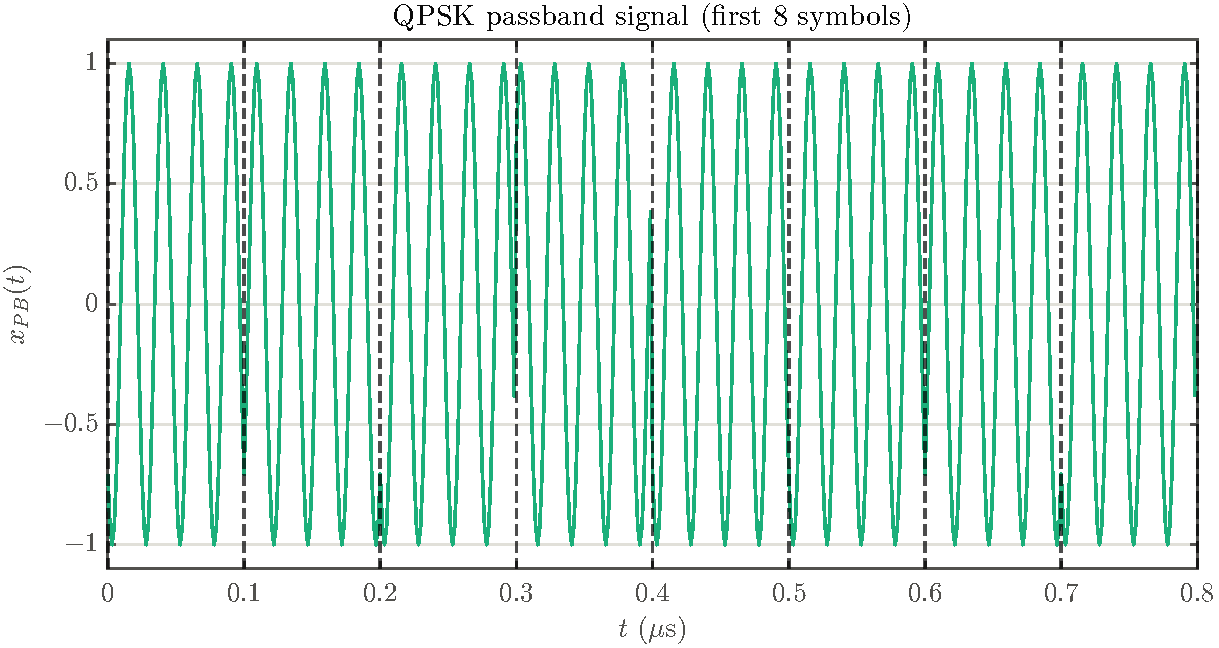
\includegraphics[width=\linewidth]{q1b.pdf}
    \caption{Passband Signal over the First Eight Symbols (black dashed lines: symbol boundaries)}
\end{figure}

\newpage

\section{(c) Baseband vs.\ Passband over Two Symbols}

\question{On a separate enlarged figure, show the baseband and passband signals over the first two symbol
periods. If both appear in one figure, identify their amplitude scales and the time scales clearly. (5\%)}

I put the two signals in separate panels with a shared time axis ($0 \sim 0.2$\,\textmu s), so each
keeps its own amplitude scale. The baseband rails sit at $\pm 1/\sqrt{2} \approx \pm 0.707$, while the
passband signal swings between $\pm 1$ because $|x_{BB}(t)| = 1$. The dots on the passband curve are the
actual samples, 16 per carrier cycle. At $t = 0.1$\,\textmu s the symbol goes from $a_0$ ($135^\circ$) to
$a_1$ ($225^\circ$). Only $Q(t)$ flips, so the carrier phase moves by $+\pi/2$.

\begin{figure}[H]
    \centering
    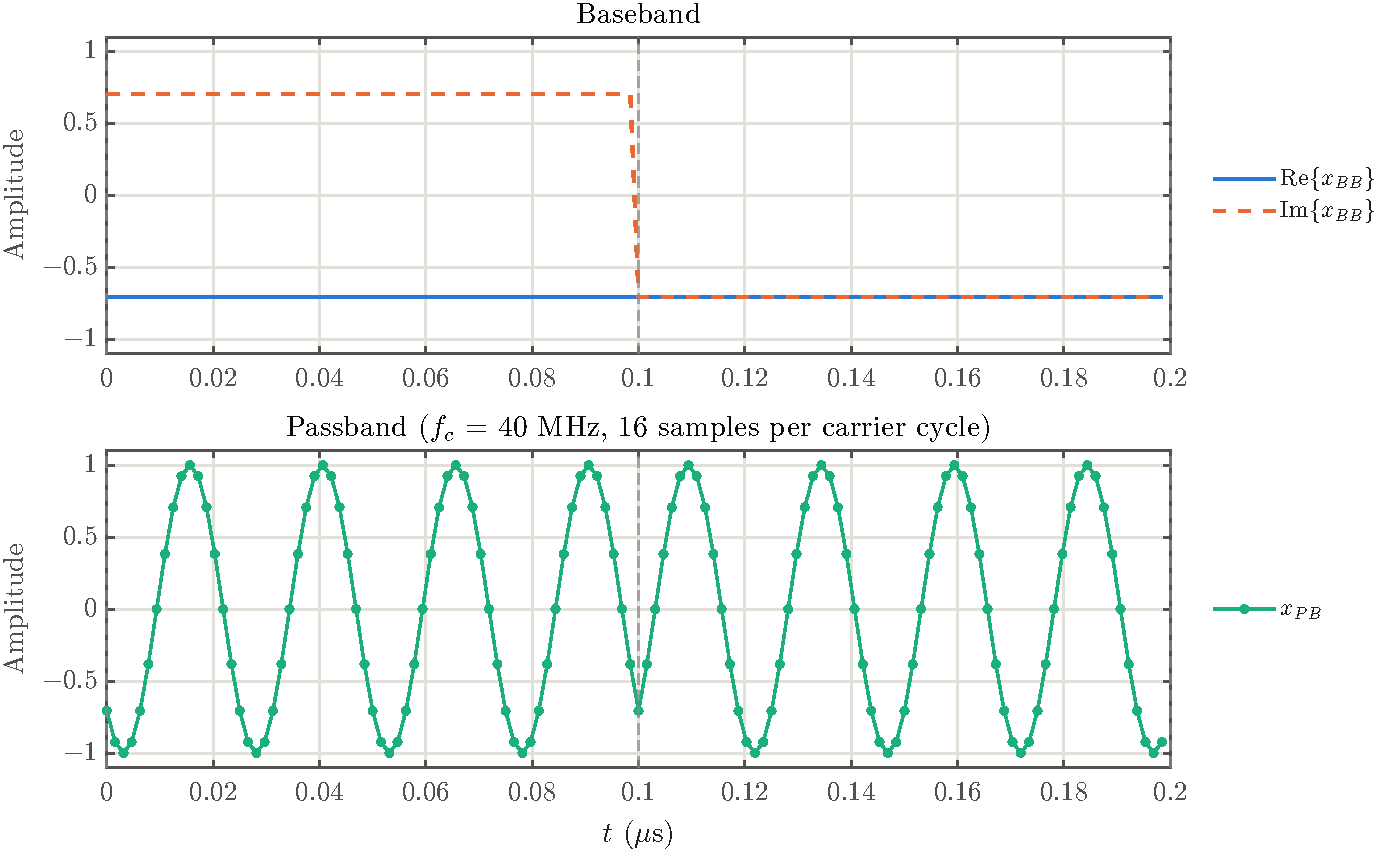
\includegraphics[width=0.95\linewidth]{q1c.pdf}
    \caption{Baseband (top) and Passband (bottom) Signals over the First Two Symbol Periods}
\end{figure}

\newpage

\section{(d) Magnitude Spectra}

\question{Use an FFT to plot the magnitude spectra of the baseband and passband signals. Use a frequency
axis in MHz. Note that the range of y-axis should be less than 60\,dB. (10\%)}

I zero-pad the 1024-sample waveforms to an 8192-point FFT (78.125\,kHz per bin) and normalize each
spectrum to its own peak. The y-axis runs from $-50$ to $+8$\,dB, a 58\,dB range.

The baseband spectrum is centered at 0\,Hz. Its envelope follows the rectangular pulse,
$|P(f)| \propto |\mathrm{sinc}(f\Tsym)|$, so the main lobe spans $\pm 10$\,MHz, the nulls fall on multiples of
$1/\Tsym = 10$\,MHz, and the first side lobe of $|P(f)|$ is 13.3\,dB below its main lobe. The fine ripples inside the envelope
come from my particular 16-symbol pattern. Because $x_{BB}(t)$ is complex, the spectrum is not symmetric about 0.

Upconversion moves this spectrum to $+f_c$ and, since the passband signal is real, adds a conjugate
mirror at $-f_c$:
\begin{equation}
    X_{PB}(f) = \tfrac{1}{2}\left[X_{BB}(f - f_c) + X_{BB}^{*}(-f - f_c)\right].
\end{equation}
The passband spectrum is therefore symmetric about 0, with its two main lobes at $\pm 40$\,MHz.

\begin{figure}[H]
    \centering
    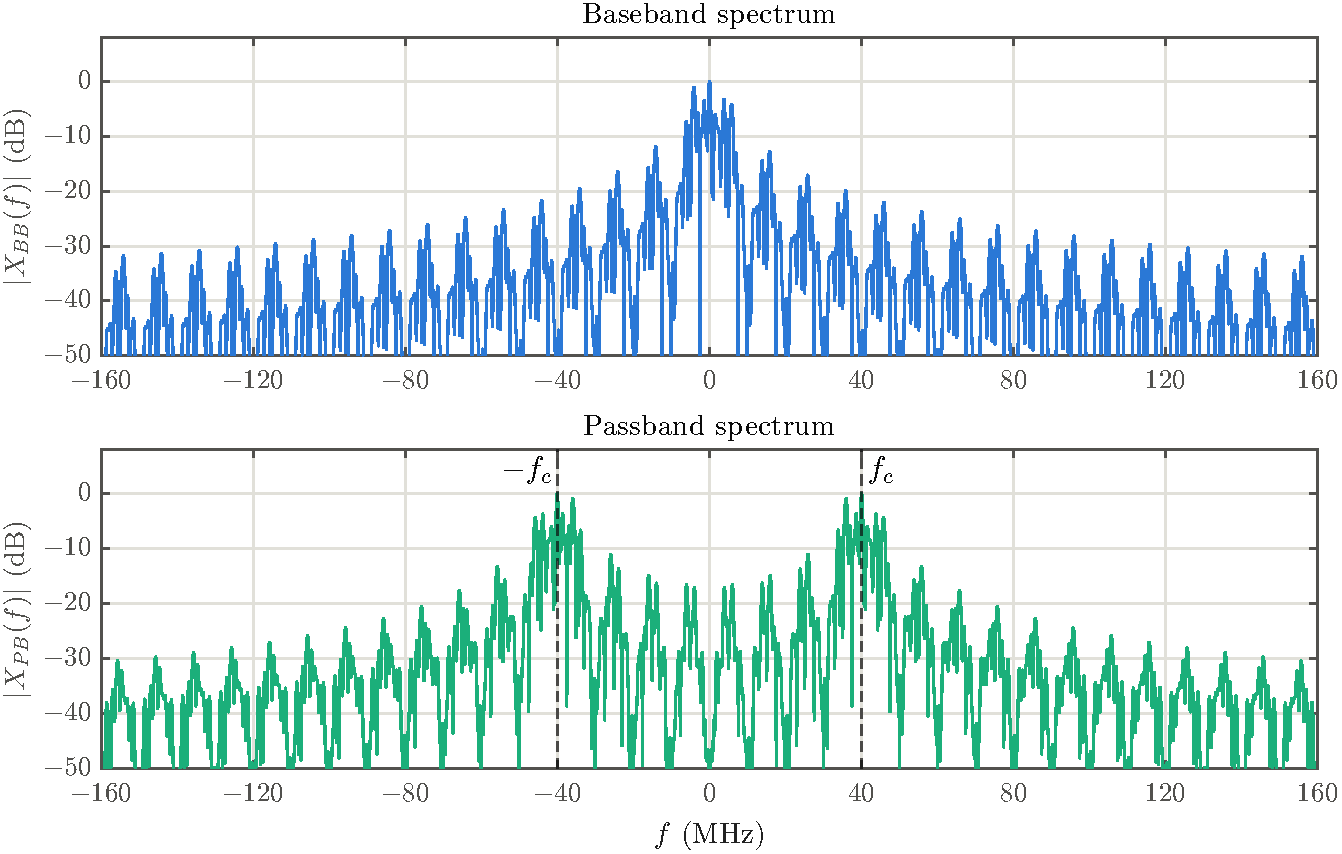
\includegraphics[width=0.95\linewidth]{q1d.pdf}
    \caption{Normalized Magnitude Spectra of the Baseband (top) and Passband (bottom) Signals}
\end{figure}

\newpage

\section{(e) O-QPSK Baseband Signal}

\question{Generate the O-QPSK baseband signal, $x_{BB,OQPSK}(t)$, by delaying the Q branch by $\Tsym/2$.
Assume $Q(t) = I(t)$ for $0 \le t < \Tsym/2$. (5\%)}

I keep the in-phase rail as it is and delay the quadrature rail by $\Tsym/2$ (32 samples):
\begin{equation}
    x_{BB,OQPSK}(t) = I(t) + j\,Q_O(t), \qquad
    Q_O(t) =
    \begin{cases}
        I(t),              & 0 \le t < \Tsym/2 \\
        Q(t - \Tsym/2),    & \Tsym/2 \le t < 16\Tsym
    \end{cases}
\end{equation}
The window stays at $0 \le t < 16\Tsym$, so the last half-symbol of $Q$ is cut off.
In the figure, $I(t)$ only switches on the dashed lines ($t = k\Tsym$) and $Q_O(t)$ only on the dotted lines
($t = (k + \tfrac{1}{2})\Tsym$). The two rails never change at the same time.

\begin{figure}[H]
    \centering
    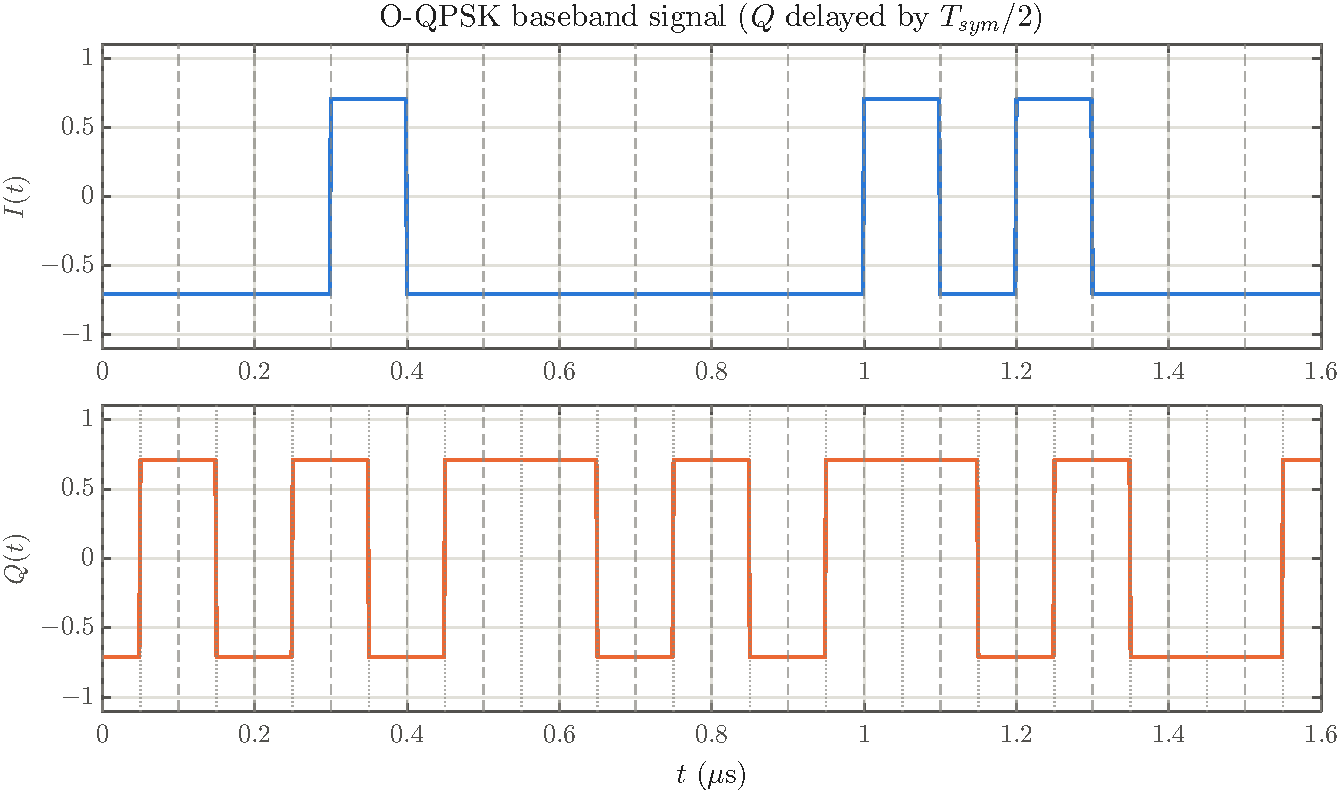
\includegraphics[width=0.9\linewidth]{q1e.pdf}
    \caption{O-QPSK Baseband Signal (dashed: $k\Tsym$, dotted: $(k+\frac{1}{2})\Tsym$)}
\end{figure}

\newpage

\section{(f) O-QPSK Phase Jump}

\question{Draw the figure of phase jump in the range of $[-\pi, \pi)$ versus $0 \le t < 16\Tsym$ for your
O-QPSK baseband signal by using ``stem''. (10\%)}

Both rails are piecewise constant, so $\angle x(t)$ can only change at the half-symbol instants
$t_m = m\Tsym/2$, $m = 0, 1, \ldots, 31$. I measure the jump at each of them as
\begin{equation}
    \Delta\phi(t_m) = \mathrm{wrap}_{[-\pi,\pi)}\left( \angle x(t_m) - \angle x(t_m^-) \right),
\end{equation}
where $t_m^-$ is the sample just before $t_m$. I set $\Delta\phi(0) = 0$ because nothing comes before $t = 0$.
Every constellation phase is an odd multiple of $\pi/4$, so every jump is a multiple of $\pi/2$, and a
jump of $\pm\pi$ shows up as $-\pi$ to stay inside $[-\pi, \pi)$. At all other samples the phase does not
change, so a sample-by-sample difference would only add zero-valued stems; the 32 instants above already
contain every non-zero jump.

\begin{figure}[H]
    \centering
    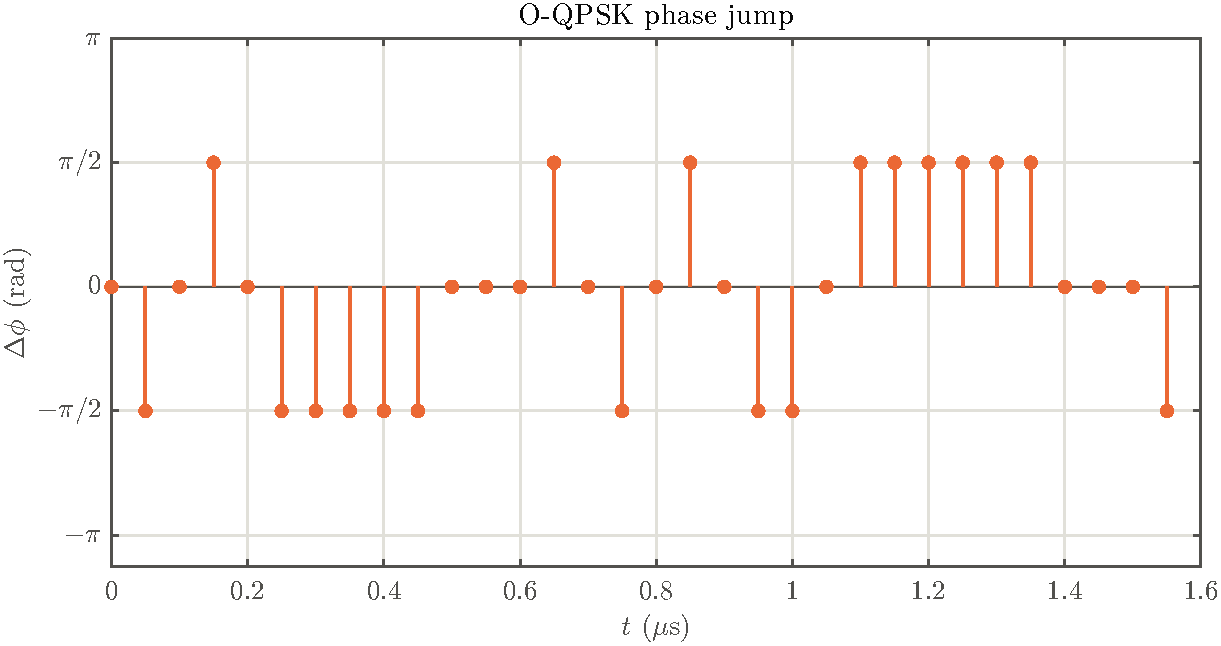
\includegraphics[width=\linewidth]{q1f.pdf}
    \caption{Phase Jump of the O-QPSK Baseband Signal}
\end{figure}

\newpage

\section{(g) Comparison with QPSK}

\question{What's your observation compared to the phase jump of the QPSK baseband signal in Q1(a)? (5\%)}

\begin{table}[H]
\centering
\caption{Phase Jump Statistics over the 32 Half-Symbol Instants}
\setlength{\tabcolsep}{14pt}
\renewcommand{\arraystretch}{1.2}
\begin{tabular}{lcccc}
\toprule
 & $-\pi$ & $-\pi/2$ & $0$ & $+\pi/2$ \\
\midrule
QPSK   & \textbf{5} & 5  & 19 & 3 \\
O-QPSK & \textbf{0} & 10 & 13 & 9 \\
\bottomrule
\end{tabular}
\end{table}

The main difference is that O-QPSK never jumps by $\pi$. In QPSK, $I$ and $Q$ can flip at the same
boundary, and when both flip the phase turns by $\pi$. With my bits this happens five times, at
$t = 0.3, 0.4, 1.1, 1.2$ and $1.3$\,\textmu s (the red stems). O-QPSK offsets the two rails by $\Tsym/2$,
so only one of them can change at any instant and $|\Delta\phi|$ never exceeds $\pi/2$.

The price is that O-QPSK jumps more often. QPSK can only change phase at $t = k\Tsym$, while O-QPSK can
change every $\Tsym/2$. Each $\pi$ jump of QPSK splits into two $\pi/2$ steps half a symbol apart: the QPSK
jump at $t = 0.30$\,\textmu s, for example, becomes an $I$ step at $0.30$\,\textmu s and a $Q$ step at
$0.35$\,\textmu s. Counting everything, the five $\pi$ jumps give ten steps, the eight $\pi/2$ jumps stay as
one step each, and one more step appears at $t = 0.05$\,\textmu s, where $Q_O(t)$ leaves the assumed value
$I(t)$ and takes the first $Q$ symbol. That makes $10 + 8 + 1 = 19$ non-zero jumps for O-QPSK, against 13 for QPSK.

Keeping the jumps small is useful in practice. A $\pi$ jump sends the signal trajectory through the origin,
and once the pulses are band-limited this shows up as a deep dip in the envelope and a higher PAPR.
With O-QPSK the envelope stays away from zero, so a nonlinear power amplifier distorts it less.
This matches the course slides (Chapter~2, pp.~21--22), which give a maximum phase shift of
$180^\circ$ for QPSK and $90^\circ$ for O-QPSK.

\begin{figure}[H]
    \centering
    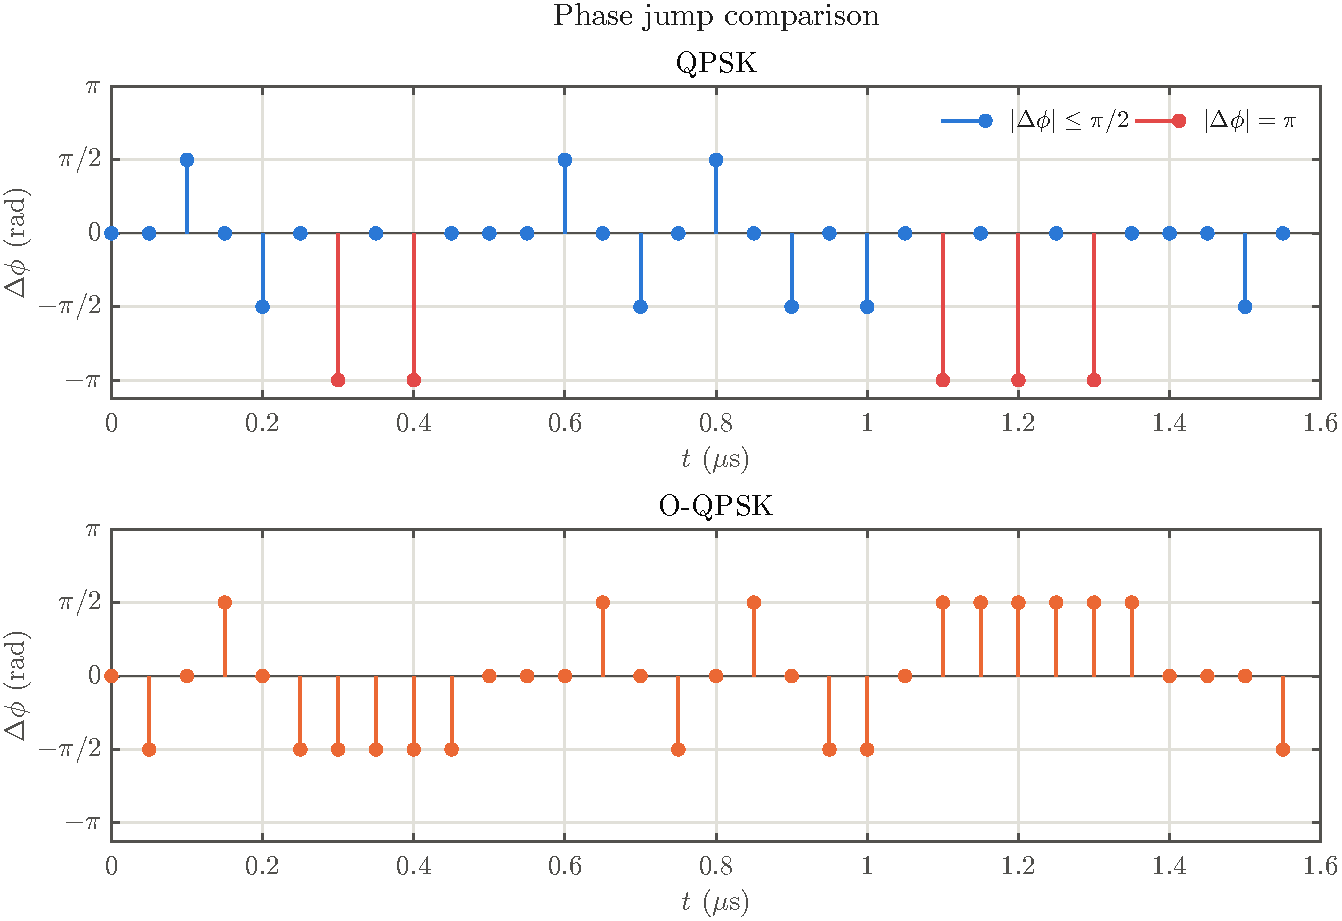
\includegraphics[width=0.85\linewidth]{q1g.pdf}
    \caption{Phase Jump Comparison: QPSK (top) vs.\ O-QPSK (bottom); red stems mark $|\Delta\phi| = \pi$}
\end{figure}

\newpage

% ─────────────────────────────────────────────
\chapter{Q2 — OFDM Baseband Signal}
% ─────────────────────────────────────────────
Q2 maps $b_0 \sim b_{31}$ to $X_k$ on all $N = 16$ subcarriers with the white points of Fig.~1:
\begin{equation}
    (0,1) \to 1, \quad (1,1) \to j, \quad (1,0) \to -1, \quad (0,0) \to -j .
\end{equation}
The baseband sample interval is $T_s = 25$\,ns.

\section{(a) Symbol Duration and Subcarrier Spacing}

\question{Calculate the useful OFDM symbol duration $\Tsym$ and the subcarrier spacing $\Delta f$. (4\%)}

\begin{equation}
    \Tsym = N T_s = 16 \times 25\,\text{ns} = \mathbf{400\,ns}, \qquad
    \Delta f = \frac{1}{\Tsym} = \frac{1}{N T_s} = \mathbf{2.5\,MHz}.
\end{equation}
This $\Delta f$ is the minimum spacing that keeps the subcarriers orthogonal, $f_{sub} = 1/(NT_s)$ in the
course slides (Chapter~2, p.~28). The sampling rate $1/T_s = 40$\,MHz is exactly $N\Delta f$, so the
16 subcarriers fill the sampled band.

\section{(b) Subcarrier Table}

\question{Create a table containing $k$, $(b_{2k}, b_{2k+1})$, $X_k$, and the signed subcarrier frequency.
Use $f_k = k\Delta f$ for $k = 0, \ldots, 7$ and $f_k = (k - N)\Delta f$ for $k = 8, \ldots, 15$. (10\%)}

\begin{table}[H]
\centering
\caption{Subcarrier Mapping and Signed Frequencies (generated by \texttt{01\_src/q2.m})}
\setlength{\tabcolsep}{8pt}
\renewcommand{\arraystretch}{1.2}
\begin{tabular}{cccr}
\toprule
$k$ & $(b_{2k}, b_{2k+1})$ & $X_k$ & $f_k$ (MHz) \\
\midrule
0 & (1, 1) & $j$ & $0.0$ \\
1 & (1, 0) & $-1$ & $+2.5$ \\
2 & (1, 1) & $j$ & $+5.0$ \\
3 & (0, 0) & $-j$ & $+7.5$ \\
4 & (1, 1) & $j$ & $+10.0$ \\
5 & (1, 1) & $j$ & $+12.5$ \\
6 & (1, 0) & $-1$ & $+15.0$ \\
7 & (1, 1) & $j$ & $+17.5$ \\
\bottomrule
\end{tabular}
\hspace{2em}
\begin{tabular}{cccr}
\toprule
$k$ & $(b_{2k}, b_{2k+1})$ & $X_k$ & $f_k$ (MHz) \\
\midrule
8 & (1, 0) & $-1$ & $-20.0$ \\
9 & (1, 1) & $j$ & $-17.5$ \\
10 & (0, 1) & $1$ & $-15.0$ \\
11 & (1, 0) & $-1$ & $-12.5$ \\
12 & (0, 1) & $1$ & $-10.0$ \\
13 & (1, 0) & $-1$ & $-7.5$ \\
14 & (1, 0) & $-1$ & $-5.0$ \\
15 & (1, 1) & $j$ & $-2.5$ \\
\bottomrule
\end{tabular}

\end{table}

\newpage

\section{(c) Individual Subcarriers $k = 1$ and $k = 14$}

\question{Let $t = uT_s/16$ for $u = 0, 1, 2, \ldots, 16N$. Generate the individual subcarrier waveforms
$y_k(t)$ versus $t$ for $k = 1$ and $14$. Plot their real and imaginary parts and verify that each subcarrier
completes the expected number of cycles during $\Tsym$. Please state how you verify it. (16\%)
\[ y_k(t) = X_k e^{j2\pi f_k t}, \quad 0 \le t < \Tsym \]}

The time grid has 257 points from $0$ to $\Tsym = 400$\,ns, spaced $T_s/16 = 1.5625$\,ns apart.
For $k = 1$, $X_1 = -1$ and $f_1 = +2.5$\,MHz, so I expect $f_1\Tsym = +1$ cycle, turning counter-clockwise.
For $k = 14$, $X_{14} = -1$ and $f_{14} = (14-16)\Delta f = -5$\,MHz, so I expect $f_{14}\Tsym = -2$ cycles,
i.e.\ two turns clockwise.

\textbf{How I verify it.} I check the cycle count in three ways in \texttt{01\_src/q2.m}:
\begin{enumerate}[label=\arabic*)]
    \item I unwrap the phase of $y_k(t)$ and divide its total change over $[0, \Tsym]$ by $2\pi$.
    This gives $+1.0000$ cycles for $k = 1$ and $-2.0000$ cycles for $k = 14$. The minus sign also
    confirms that the negative frequency turns clockwise.
    \item I count zero crossings. One full cycle crosses zero twice, and $\mathrm{Re}\{y_1(t)\}$ and
    $\mathrm{Re}\{y_{14}(t)\}$ cross zero 2 and 4 times, which is $2|f_k\Tsym|$ in both cases.
    \item A whole number of cycles means $y_k(\Tsym) = y_k(0)$. The measured $|y_k(\Tsym) - y_k(0)|$ is
    $2.4 \times 10^{-16}$ and $4.9 \times 10^{-16}$, which is zero up to double precision.
\end{enumerate}
The plot agrees: $y_1$ goes through one period, and $y_{14}$ repeats at $t = 200$\,ns (dotted line).
For $k = 14$, $\mathrm{Im}\{y_{14}\}$ leads $\mathrm{Re}\{y_{14}\}$ by a quarter period, which is what a
phasor turning clockwise looks like.

\begin{figure}[H]
    \centering
    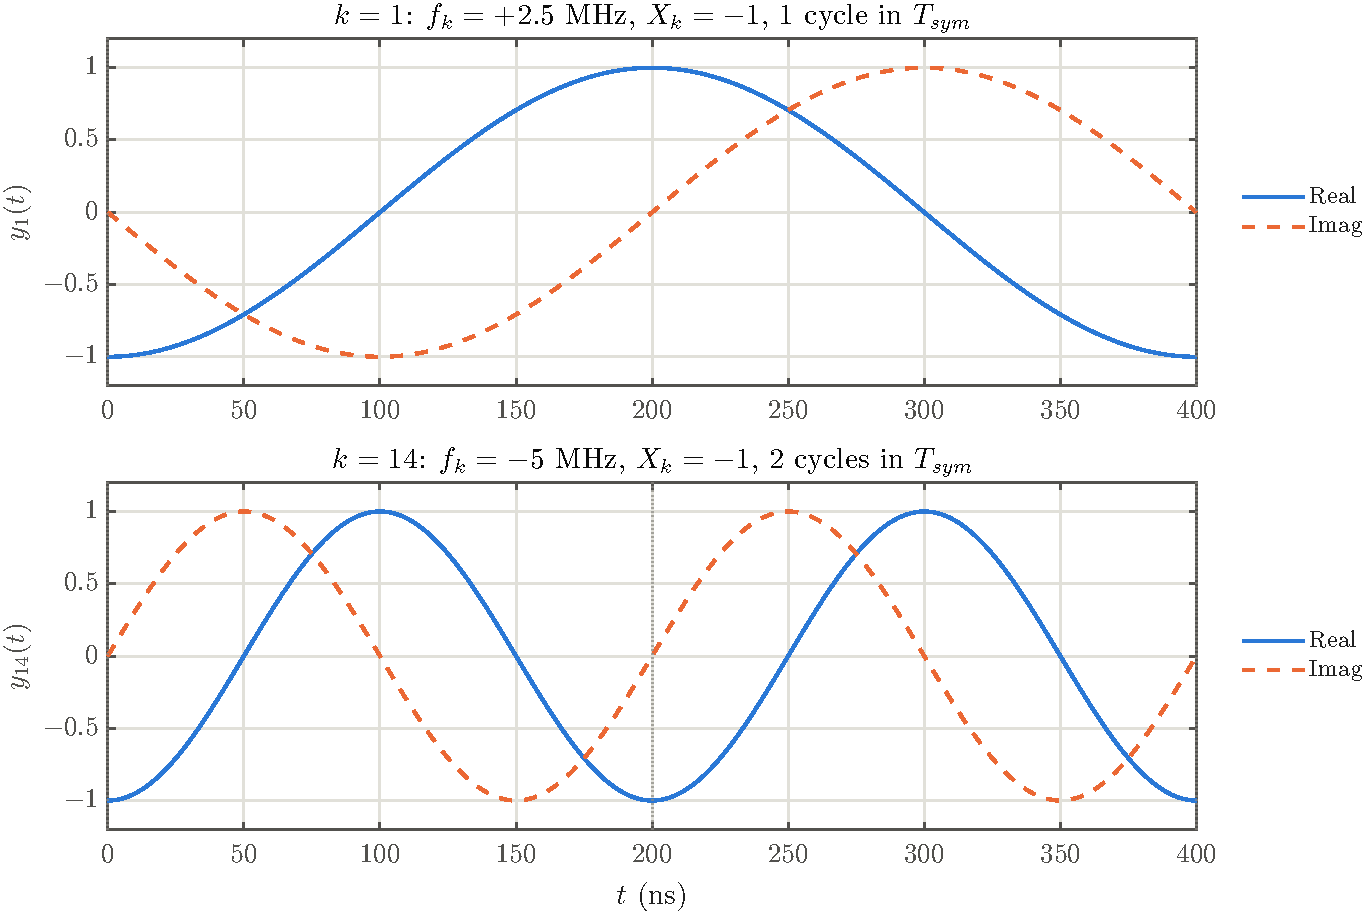
\includegraphics[width=\linewidth]{q2c.pdf}
    \caption{Subcarrier Waveforms $y_1(t)$ (top) and $y_{14}(t)$ (bottom)}
\end{figure}

\newpage

\section{(d) Sum of All Subcarriers}

\question{Sum all 16 subcarrier waveforms. Plot the real part and imaginary part of $y(t)$ versus $t$. (5\%)
\[ y(t) = \sum_{k=0}^{N-1} X_k e^{j2\pi f_k t} \]}

An easy point to check is $t = 0$, where $y(0) = \sum_k X_k$. The table has seven $j$, one $-j$,
six $-1$ and two $+1$, so $y(0) = -4 + 6j$, and that is where both curves start.
Every $f_k\Tsym$ is an integer, so $y(t)$ comes back to $-4 + 6j$ at $t = \Tsym$.

\begin{figure}[H]
    \centering
    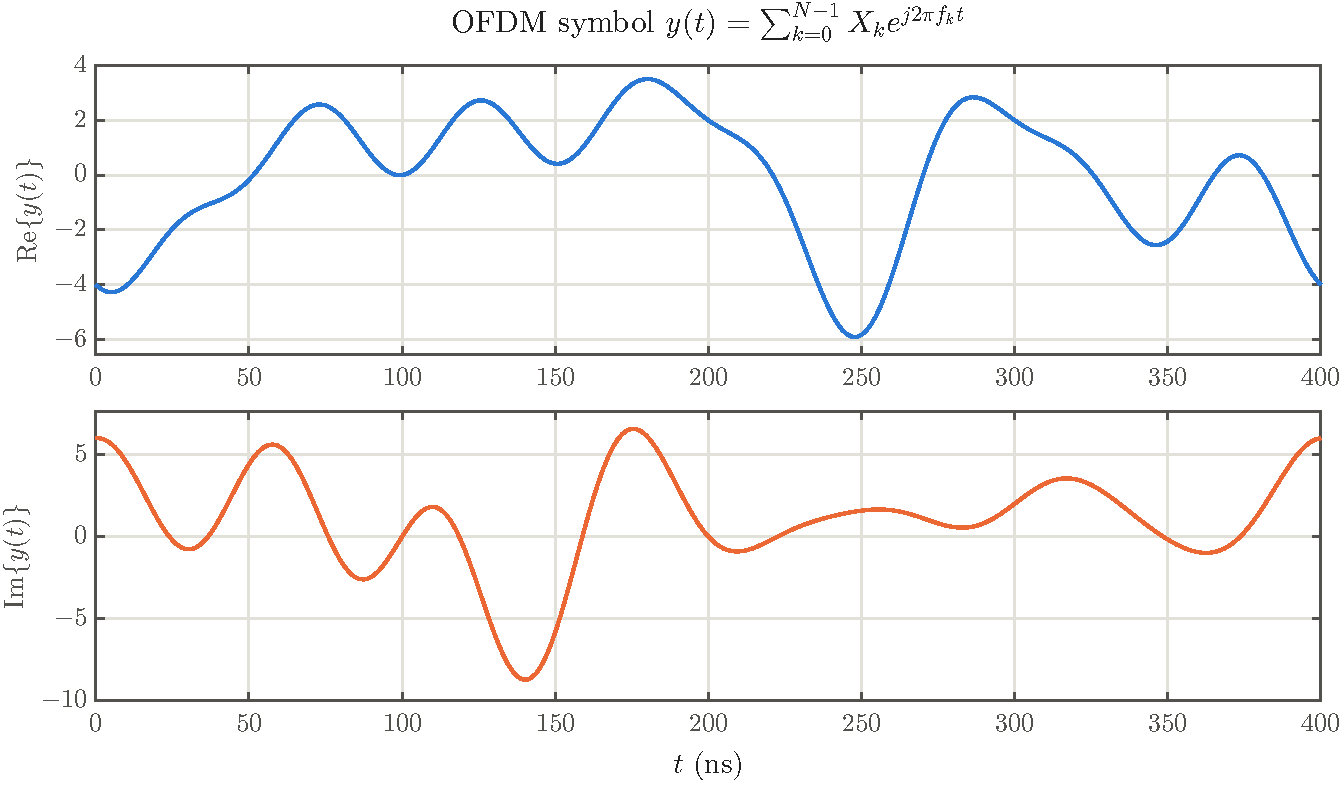
\includegraphics[width=0.95\linewidth]{q2d.pdf}
    \caption{Real and Imaginary Parts of the OFDM Symbol $y(t)$}
\end{figure}

\newpage

\section{(e) 16-Point IFFT}

\question{Now, calculate $x[n]$ using the 16-point IFFT definition below. Please use ``stem'' to draw the
discrete samples $Nx[n]$ and plot $y(t)$ in the same figure for the real part and imaginary part. (10\%)
\[ x[n] = \frac{1}{N}\sum_{k=0}^{N-1} X_k e^{j2\pi kn/N}, \quad n = 0, \ldots, N-1 \]}

I compute $x[n]$ with MATLAB \texttt{ifft}, which already includes the $1/N$ factor, and compare it with
the definition above written out as a direct sum; the two differ by at most $9.0 \times 10^{-16}$.
Placing $Nx[n]$ at $t = nT_s$, every stem lands on the continuous curve. In numbers,
\begin{equation}
    \max_n \left| N x[n] - y(nT_s) \right| = 1.6 \times 10^{-14}.
\end{equation}

\begin{figure}[H]
    \centering
    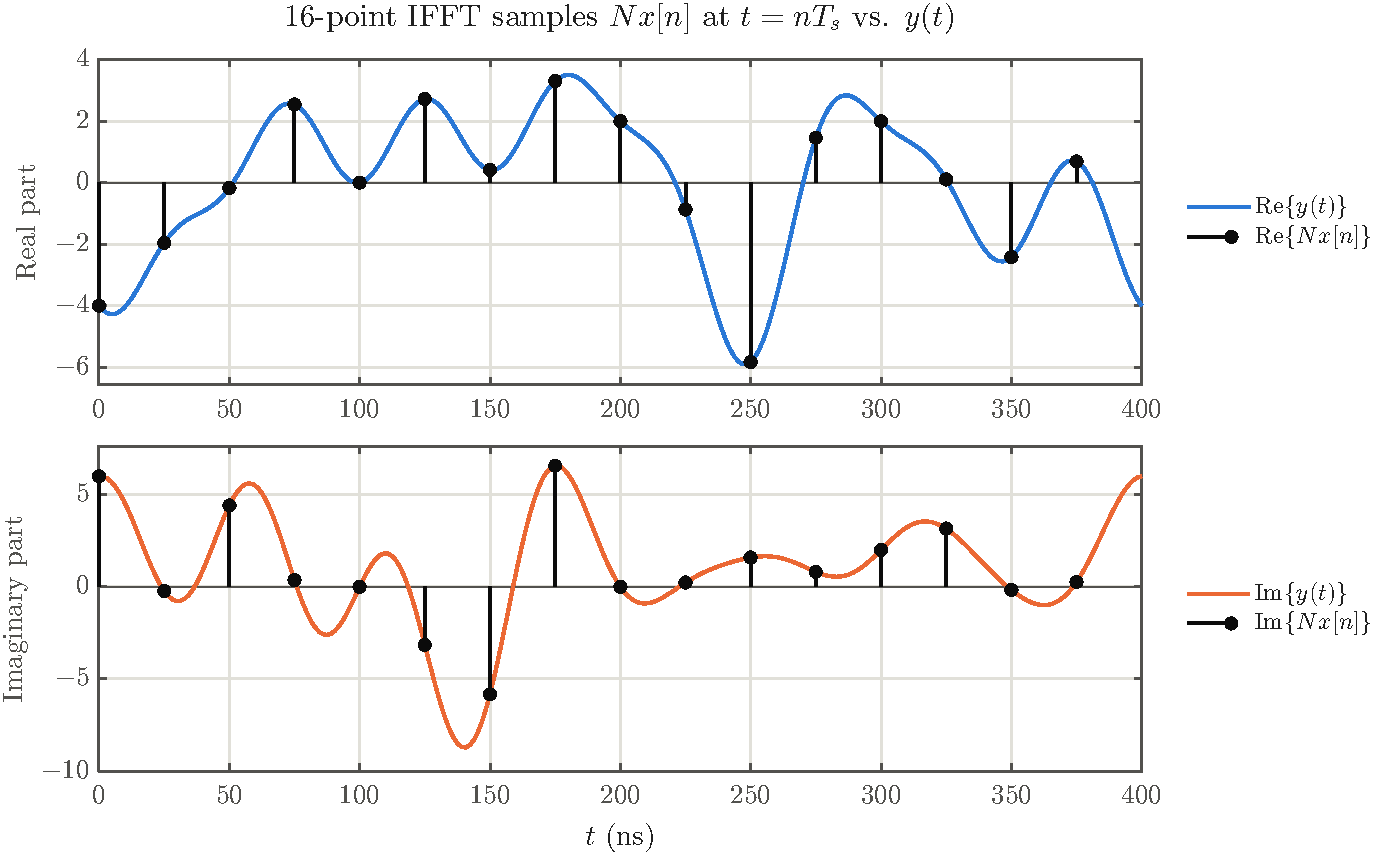
\includegraphics[width=0.95\linewidth]{q2e.pdf}
    \caption{IFFT Samples $Nx[n]$ (stems) and the Continuous Signal $y(t)$}
\end{figure}

\newpage

\section{(f) Signed vs.\ Unsigned Subcarrier Frequencies}

\question{In Q2(b) and Q2(d), we use $f_k = (k - N)\Delta f$ for $k \ge 8$, but for generating $x[n]$,
$k\Delta f$ is assumed for $k \ge 8$. Although we use different frequency values, actually the discrete
samples $Nx[n]$ have the same magnitude of the real part and imaginary part as those of $y(nT_s)$. Why? (5\%)}

The two frequencies differ by exactly the sampling rate, $N\Delta f = 1/T_s$, so they are aliases of each
other and look identical at the sampling instants. Using $\Delta f\, T_s = 1/N$, for $k \ge 8$:
\begin{equation}
    e^{j2\pi (k-N)\Delta f \cdot nT_s}
    = e^{j2\pi (k-N) n / N}
    = e^{j2\pi kn/N}\, \underbrace{e^{-j2\pi n}}_{=\,1}
    = e^{j2\pi kn/N}.
\end{equation}
So each term of $y(nT_s)$ equals the matching term of the IDFT, and $y(nT_s) = \sum_k X_k e^{j2\pi kn/N} = N x[n]$.
The two are not just equal in magnitude; the real and imaginary parts match exactly.
In my simulation, $\max_n |y_{\text{signed}}(nT_s) - y_{\text{unsigned}}(nT_s)| = 2.2 \times 10^{-14}$.

Between the samples, though, they are different signals, and on the fine grid they differ by up to 10.65.
The signed version keeps every subcarrier inside $[-N/2, N/2)\Delta f$. That makes it the smooth, band-limited
waveform a DAC and low-pass filter would rebuild from $x[n]$. The unsigned version reaches up to
$15\Delta f = 37.5$\,MHz and wiggles much faster in between.

\begin{figure}[H]
    \centering
    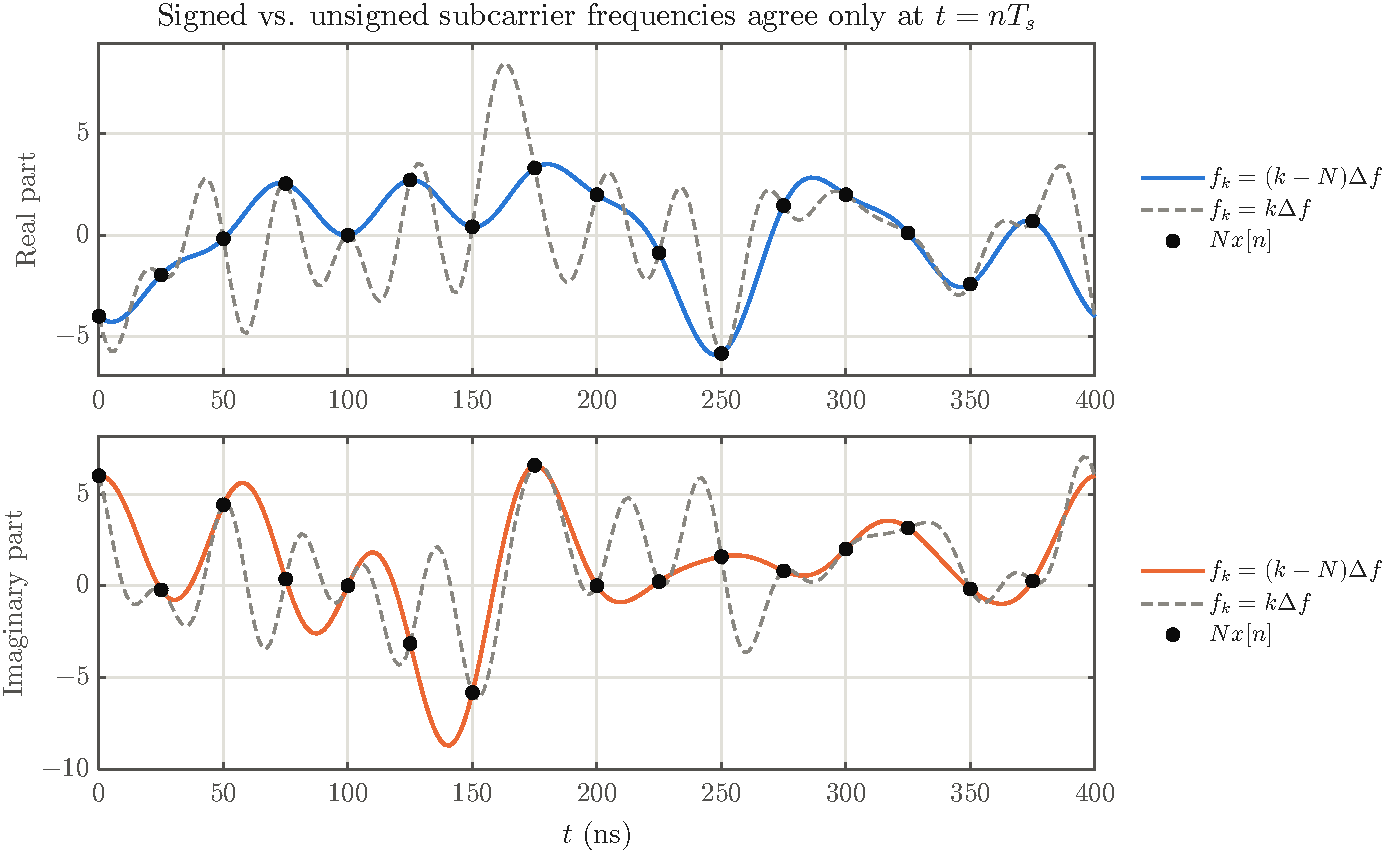
\includegraphics[width=0.95\linewidth]{q2f.pdf}
    \caption{Signed ($f_k = (k-N)\Delta f$) and Unsigned ($f_k = k\Delta f$) Waveforms Agree Only at $t = nT_s$}
\end{figure}

\newpage

% ─────────────────────────────────────────────
\chapter{Q3 — OTFS Baseband Signal}
% ─────────────────────────────────────────────
Q3 uses $N = 4$ Doppler bins (time slots) and $M = 8$ delay bins (subcarriers), with BPSK symbols
\begin{equation}
    X_{DD}[l, k] = 1 - 2b_i, \qquad i = kM + l, \quad 0 \le l \le M-1,\ 0 \le k \le N-1.
\end{equation}
A note on indexing: the spec writes $X_{DD}[l,k]$ in the mapping but $X_{DD}[k,l]$ inside the ISFFT.
I follow the course slides (Chapter~2, p.~44), which write $x_{DD}[l,k]$ with $l$ on the delay axis and
$k$ on the Doppler axis, so both expressions refer to the same grid. The exponent $nk/N - ml/M$ also pairs
$k$ with $N$ and $l$ with $M$, which leaves no other reading. In MATLAB the grid is \texttt{reshape(1-2*b, M, N)}.

\begin{table}[H]
\centering
\caption{Delay-Doppler Grid $X_{DD}[l, k]$}
\setlength{\tabcolsep}{12pt}
\renewcommand{\arraystretch}{1.1}
\begin{tabular}{c|rrrr}
\toprule
$l \backslash k$ & 0 & 1 & 2 & 3 \\
\midrule
0 & $-1$ & $-1$ & $-1$ & $+1$ \\
1 & $-1$ & $-1$ & $+1$ & $-1$ \\
2 & $-1$ & $-1$ & $-1$ & $-1$ \\
3 & $+1$ & $-1$ & $-1$ & $+1$ \\
4 & $-1$ & $-1$ & $+1$ & $-1$ \\
5 & $-1$ & $+1$ & $-1$ & $+1$ \\
6 & $+1$ & $-1$ & $-1$ & $-1$ \\
7 & $+1$ & $-1$ & $+1$ & $-1$ \\
\bottomrule
\end{tabular}
\end{table}

\newpage

\section{(a) ISFFT: Delay-Doppler to Time-Frequency}

\question{First, apply ISFFT to change the signal from the delay-Doppler domain to the time-frequency domain.
Plot the real part and imaginary part of the time-frequency grid $X_{TF}[0, m]$ and $X_{TF}[2, m]$ with labeled
subcarrier index $m$. (10\%)
\[ X_{TF}[n, m] = \frac{1}{\sqrt{NM}} \sum_{k=0}^{N-1} \sum_{l=0}^{M-1} X_{DD}[k, l]\, e^{j2\pi\left(\frac{nk}{N} - \frac{ml}{M}\right)} \]}

The ISFFT is an $N$-point IDFT along the Doppler index $k$ combined with an $M$-point DFT along the delay
index $l$. I implement it as a matrix product, $X_{TF} = F_N X_{DD}^{T} F_M / \sqrt{NM}$ with
$[F_N]_{n,k} = e^{j2\pi nk/N}$ and $[F_M]_{l,m} = e^{-j2\pi ml/M}$, and compare it with the double sum above
computed element by element. They differ by at most $1.5 \times 10^{-15}$.

\begin{table}[H]
\centering
\caption{Time-Frequency Samples $X_{TF}[0, m]$ and $X_{TF}[2, m]$}
\setlength{\tabcolsep}{14pt}
\renewcommand{\arraystretch}{1.1}
\begin{tabular}{crr}
\toprule
$m$ & $X_{TF}[0, m]$ & $X_{TF}[2, m]$ \\
\midrule
0 & $-2.1213$            & $0.7071$ \\
1 & $-0.2500 + 0.6036j$  & $0.5429 + 0.1036j$ \\
2 & $0.3536 + 0.3536j$   & $-0.3536 + 1.0607j$ \\
3 & $0.2500 - 0.1036j$   & $-1.9571 - 0.6036j$ \\
4 & $-1.4142$            & $0$ \\
5 & $0.2500 + 0.1036j$   & $-1.9571 + 0.6036j$ \\
6 & $0.3536 - 0.3536j$   & $-0.3536 - 1.0607j$ \\
7 & $-0.2500 - 0.6036j$  & $0.5429 - 0.1036j$ \\
\bottomrule
\end{tabular}
\end{table}

The table has a pattern worth pointing out. Since $X_{DD}$ is real, $X_{TF}[n, m]^{*} = X_{TF}[-n, -m]$,
and for $n = 0$ and $n = 2$ we have $-n \equiv n \bmod 4$, so $X_{TF}[n, M-m] = X_{TF}[n, m]^{*}$.
Both rows are indeed conjugate-symmetric around $m = 4$, and the entries at $m = 0$ and $m = 4$ are real.

\begin{figure}[H]
    \centering
    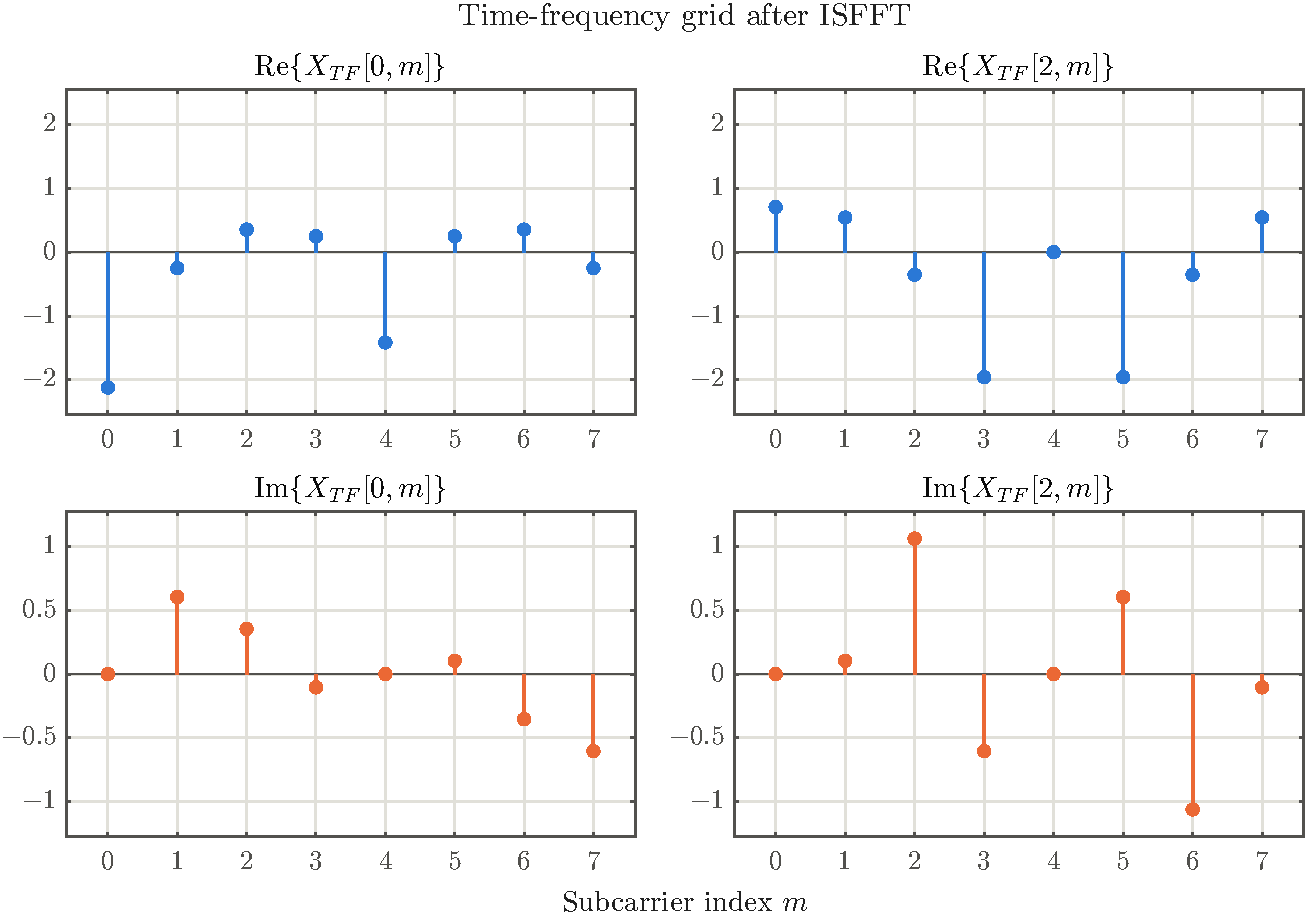
\includegraphics[width=0.95\linewidth]{q3a.pdf}
    \caption{Real (top) and Imaginary (bottom) Parts of $X_{TF}[0, m]$ (left) and $X_{TF}[2, m]$ (right)}
\end{figure}

\newpage

\section{(b) Delay-Time Domain and Time-Domain Signal}

\question{Next, change the signal from the time-frequency domain $X_{TF}[n, m]$ to the delay-time domain
$X_{DT}[n, l]$ by applying a unitary IFFT along the frequency-domain subcarrier index $m$, just like your OFDM system,
and repeat for every time index $n = 0, 1, 2, 3$. Then rearrange the delay-time domain signal into the
one-dimensional time-domain signal $x[q]$, where $q = nM + l$. Plot the real part and imaginary part of $x[q]$. (10\%)}

For every time slot $n$, the unitary $M$-point IFFT is
\begin{equation}
    X_{DT}[n, l] = \frac{1}{\sqrt{M}} \sum_{m=0}^{M-1} X_{TF}[n, m]\, e^{j2\pi ml/M},
\end{equation}
which is \texttt{ifft(Xtf, M, 2) * sqrt(M)} in MATLAB. I then place the rows one after another in time,
$x[nM + l] = X_{DT}[n, l]$.

\begin{table}[H]
\centering
\caption{Time-Domain Samples $x[q]$, $q = nM + l$}
\label{tab:xq}
\setlength{\tabcolsep}{14pt}
\renewcommand{\arraystretch}{1.1}
\begin{tabular}{c|rrrr}
\toprule
$l \backslash n$ & 0 & 1 & 2 & 3 \\
\midrule
0 & $-1$ & $-j$    & $-1$ & $j$ \\
1 & $-1$ & $-1$    & $1$  & $-1$ \\
2 & $-2$ & $0$     & $0$  & $0$ \\
3 & $0$  & $1 - j$ & $0$  & $1 + j$ \\
4 & $-1$ & $-1$    & $1$  & $-1$ \\
5 & $0$  & $0$     & $-2$ & $0$ \\
6 & $-1$ & $1$     & $1$  & $1$ \\
7 & $0$  & $0$     & $2$  & $0$ \\
\bottomrule
\end{tabular}
\end{table}

\begin{figure}[H]
    \centering
    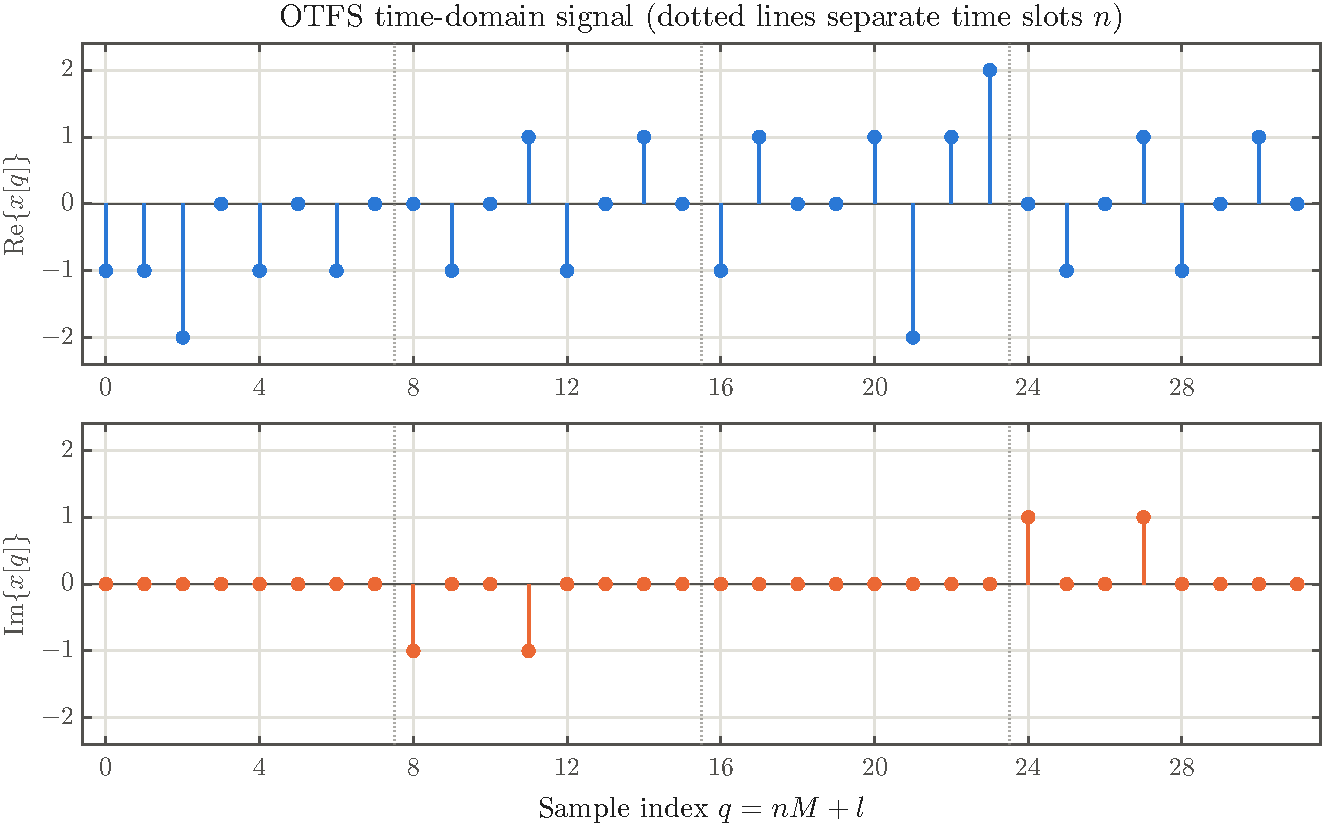
\includegraphics[width=0.85\linewidth]{q3b.pdf}
    \caption{Real (top) and Imaginary (bottom) Parts of $x[q]$ (dotted lines separate the time slots $n$)}
\end{figure}

\newpage

\section{(c) Verification}

\question{How do you know whether your result is correct or not? Please show your verification. (10\%)}

I check the result in three ways.

\textbf{1) Closed form.} If I substitute the ISFFT into the IFFT along $m$, the DFT along $l$ and the IDFT
along $m$ cancel each other:
\begin{align}
    X_{DT}[n, l]
    &= \frac{1}{\sqrt{N}} \sum_{k=0}^{N-1} \sum_{l'=0}^{M-1} X_{DD}[l', k]\, e^{j2\pi nk/N}
       \underbrace{\frac{1}{M} \sum_{m=0}^{M-1} e^{j2\pi m(l - l')/M}}_{=\,\delta[l - l']}
     = \frac{1}{\sqrt{N}} \sum_{k=0}^{N-1} X_{DD}[l, k]\, e^{j2\pi nk/N}.
\end{align}
What is left is a unitary $N$-point IDFT along the Doppler axis for each delay $l$, which is the inverse
Zak transform. This form is easy to check by hand. For example, $x[0] = \tfrac{1}{2}(-1-1-1+1) = -1$,
$x[2] = \tfrac{1}{2}(-1-1-1-1) = -2$ and $x[8] = \tfrac{1}{2}(-1 - j + 1 - j) = -j$, all of which match
Table~\ref{tab:xq}. Across all 32 samples, $\max_q |x[q] - x_{\text{closed}}[q]| = 2.1 \times 10^{-15}$.

\textbf{2) Round trip.} I run the receiver side in reverse: reshape $x[q]$ back into $X_{DT}[n, l]$, take the
unitary FFT along $l$ to get $X_{TF}$, and apply the SFFT from the course slides (Chapter~2, p.~43) to
return to the delay-Doppler grid. The recovered
grid matches the transmitted one to within $1.8 \times 10^{-15}$, with an imaginary residue of
$8.2 \times 10^{-16}$, and hard decisions give back all 32 bits with no errors.

\textbf{3) Energy.} Every step is unitary, so by Parseval's theorem $\sum|X_{DD}|^2$, $\sum|X_{TF}|^2$ and
$\sum|x[q]|^2$ must be equal. All three come out to $32.0000$, the energy of $NM = 32$ unit BPSK symbols.

\begin{figure}[H]
    \centering
    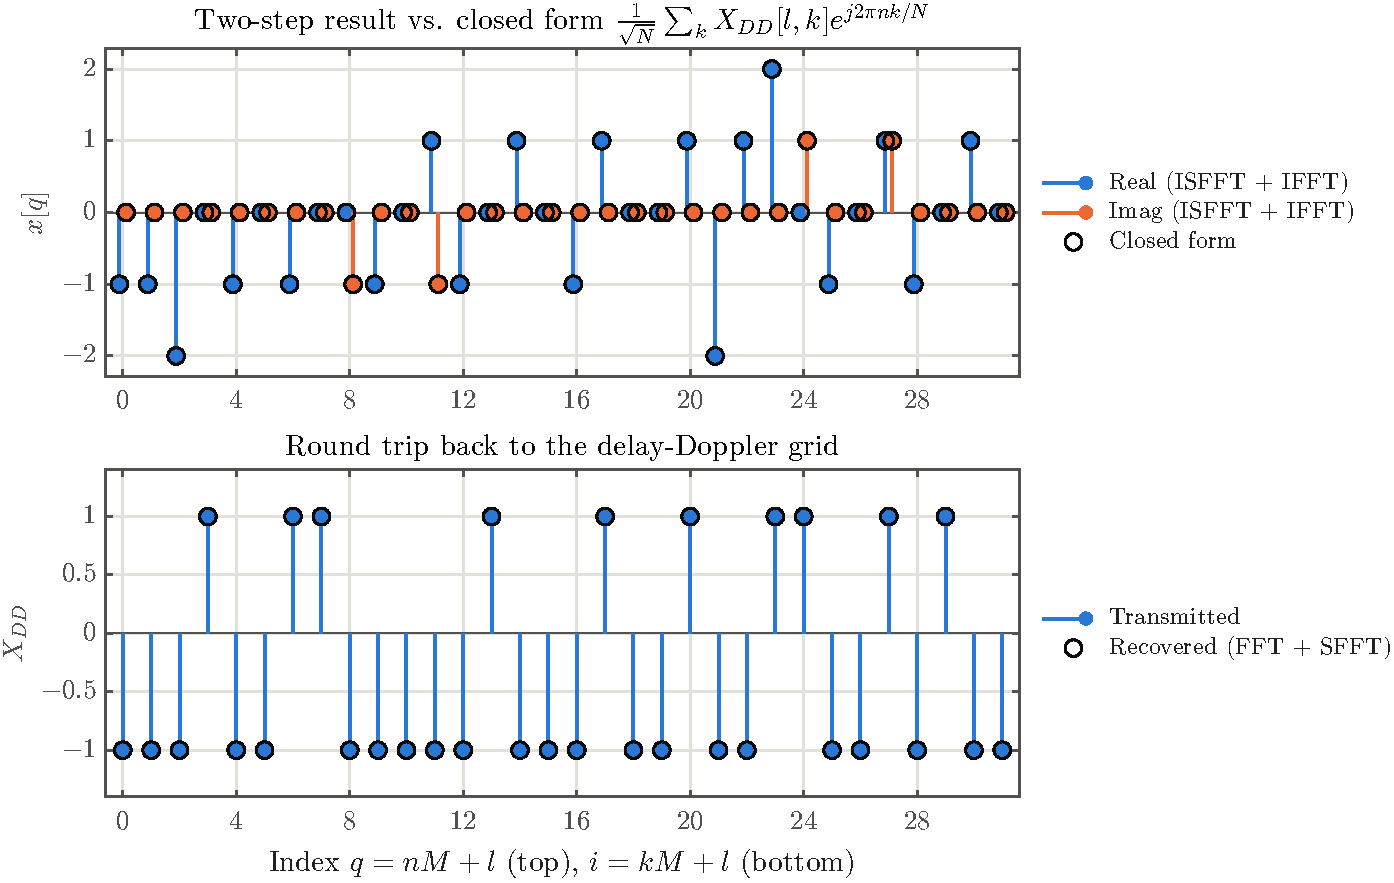
\includegraphics[width=0.95\linewidth]{q3c.pdf}
    \caption{Verification: Two-Step Result vs.\ Closed Form (top) and Round Trip back to $X_{DD}$ (bottom)}
\end{figure}

\newpage

% ─────────────────────────────────────────────
\chapter{AI Tool Disclosure}
\label{ch:ai}
% ─────────────────────────────────────────────
\question{Please disclose how you use AI tools and its version.}

I used \textbf{Claude Opus 5.5} to help with this homework in the following four parts:
\begin{enumerate}[label=(\arabic*)]
    \item Understanding the homework specification.
    \item Assisting with the MATLAB code.
    \item Plotting the figures.
    \item Writing this \LaTeX{} report.
\end{enumerate}

\end{document}
